%=====================================================================
\section{R in Action}
%=====================================================================

\begin{frame}
	\frametitle{Outline}
	
	\begin{columns}
		\column{0.5\textwidth}
		\begin{block}{Refresh R skills}
		\end{block}
		
		\column{0.5\textwidth}
		
\includegraphics[width=0.3\textwidth]{../figs/Rlogo.png}
	\end{columns}

	\vfill
	
	\begin{columns}[onlytextwidth]
		\column{0.5\textwidth}
		\begin{block}{Data Analysis}
			\begin{itemize}
				\item Base R
				\item The pipe
				\item dplyr
				\item ggplot2
				\item R Markdown
			\end{itemize}
		\end{block}

		\column{0.5\textwidth}
		\begin{block}{Writing Functions}
			\begin{itemize}
				\item Why functions?
				\item Code style
				\item Organization
				\item dplyr and ggplot2
				\item plot, print, summary
			\end{itemize}
		\end{block}
	\end{columns}
\end{frame}

%=====================================================================
\subsection{Data Analysis}
%=====================================================================

\begin{frame}
	\frametitle{Data Analysis}
	
	\begin{itemize}
		\item Throughout the lecture, we will work with R
		\item Today, focus is on \alert{data preparation} and \alert{descriptive analysis}
		\item Essential part of every analysis
		\item Base R has hundreds of functions to help you here
	\end{itemize}

	\begin{columns}
		\column{0.3\textwidth}
		\column{0.2\textwidth}
		\begin{example}
		\end{example}
		\column{0.2\textwidth}
		
\includegraphics[width=0.95\textwidth]{pics/diamond.jpg}
		\column{0.3\textwidth}
	\end{columns}

	\begin{block}{Contributed extension packages help as well. Let's look at some of them \dots}
	\end{block}

\end{frame}

\begin{frame}
	\frametitle{The Pipe Operator avoids Function Chains}
	\begin{columns}
		\column{0.5\textwidth}
		\centering
\includegraphics[width=0.25\textwidth]{../figs/magrittr.png}
		
		\begin{itemize}
			\item In ``magrittr'' package
			\item On CRAN since 2014 
			
			(Stefan Milton Bache)
			\item Turns \ttfamily{f(x, y)} into \ttfamily{x \%>\% f(y)}
			\item Since R 4.1, ``|>'' in base R
			\item Use short-cut ``Ctrl-shift-m''
		\end{itemize}
		\begin{example}
		\end{example}
		\column{0.5\textwidth}
		\begin{figure}
			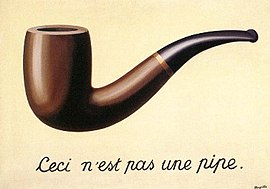
\includegraphics[width=0.9\textwidth]{pics/MagrittePipe.jpg}
			\caption{\url{https://en.wikipedia.org/wiki/The_Treachery_of_Images}}
		\end{figure}
	\end{columns}
\end{frame}

\begin{frame}
	\frametitle{``dplyr'': Grammar of Data Manipulation}
	\begin{columns}[onlytextwidth]
		\column{0.3\textwidth}
		\hspace*{0.5cm}
\includegraphics[width=0.4\textwidth]{../figs/dplyr.png}
		\begin{block}{Core ``verbs''}
			\begin{itemize}
				\item \ttfamily{select()}
				\item \ttfamily{filter()}
				\item \ttfamily{arrange()}
				\item \ttfamily{mutate()}
				\item \ttfamily{summarize()}
			\end{itemize}
		\end{block}
		
		\column{0.7\textwidth}
		\begin{block}{Dream team with pipe}
			\begin{itemize}
				\item Verbs take as first argument a dataframe and return modified dataframe
				\item On CRAN since 2014 (Hadley Wickham)
				\item Like ``magrittr'', part of tidyverse
				\item Translate between base R and dplyr?
			\end{itemize}
		\end{block}

		\begin{example}
		\end{example}
	\end{columns}
\end{frame}

\begin{frame}
	\frametitle{``ggplot2'': Grammar of Graphics}
	\begin{columns}
		\column{0.5\textwidth}
		\centering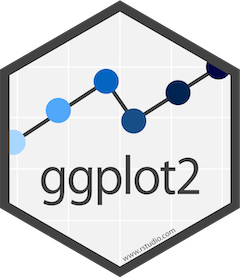
\includegraphics[width=0.3\textwidth]{../figs/ggplot2.png}
	
		\begin{block}{Modify plot layer per layer}
			\begin{itemize}
				\item Simple ``{\ttfamily +}'' instead of {\ttfamily \%>\%}
				\item On CRAN since 2007 
				
				(Hadley Wickham)
				\item Also in tidyverse
			\end{itemize}
		\end{block}
	
		\column{0.5\textwidth}
		\begin{block}{``plotly'' package}
			\begin{itemize}
				\item Interactive figures
				\item Wraps JavaScript library
				\item Can translate ggplot to Plotly
			\end{itemize}
		\end{block}
	
		\begin{example}
		\end{example}
	\end{columns}
	
\end{frame}

\begin{frame}
	\frametitle{Reports with R Markdown}
	\begin{columns}
		\column{0.4\textwidth}
		\hspace{1cm}
\includegraphics[width=0.3\textwidth]{../figs/rmarkdown.png}
		\begin{block}{Markdown text + R code}
			$\rightarrow$ HTML, Word, PDF
			
			On CRAN since 2014 (Yihui Xie)		
		\end{block}			
		
		\begin{example}
			\begin{itemize}
				\item Markdown syntax
				\item Simple R Markdown file
			\end{itemize}
		\end{example}
		
		\column{0.6\textwidth}
		\begin{block}{Workflow}
			\begin{enumerate}
				\item Create .Rmd with YAML header
				\item Write analysis and adapt YAML
				\item Hit ``Knit''/\texttt{rmarkdown::render()}
			\end{enumerate}
		\end{block}
	
		\begin{block}{When you hit ``Knit''}
			\begin{enumerate}
				\item \texttt{knitr::knit()} searchs code chunks, runs them and ``knits'' the results with your Markdown text to a temporary .md file
				\item The .md file is converted to desired output with Pandoc, using YAML header to specify its call 
			\end{enumerate}
		\end{block}
	
	\end{columns}
\end{frame}

%=====================================================================
\subsection{Writing Functions}
%=====================================================================

\begin{frame}
	\frametitle{Writing Functions}
	\begin{columns}
		\column{0.5\textwidth}
		\begin{block}{Already used many functions}
			\begin{itemize}
				\item \texttt{mean()}
				\item \texttt{ggplot2::ggplot()}
				\item \texttt{+}
			\end{itemize}
		\end{block}
	
		\begin{block}{Write \alert{own} functions to}
			\begin{itemize}
				\item avoid code duplication
				\item produce readable code
			\end{itemize}
			\begin{example}
			\end{example}
		\end{block}
	
		\column{0.5\textwidth}
		\begin{block}{Code style}
			\begin{itemize}
				\item Line length, curly braces, spaces?
				\item Comments: Why, not what
				\item Defensive programming: \texttt{if} + \texttt{stop()}
			\end{itemize}
		
			\begin{example}
			\end{example}
		\end{block}
		
		\begin{block}{Organizing functions}
			\texttt{source(functions.R)} or \alert{own package}
			\begin{example}
			\end{example}
		\end{block}
	\end{columns}
\end{frame}

\begin{frame}
	\frametitle{dplyr and ggplot2 in functions}

	\begin{block}{Unquoted variable names look nice}
		\begin{itemize}
			\item \texttt{diamonds \%>\% select(price, color)}
			\item \texttt{ggplot(diamonds, aes(x = color))}
			\item \texttt{facet\_grid($\sim$ color)}
		\end{itemize}
	\end{block}
	
	But what if ``price'' and/or ``color'' should be passed as function arguments?
	
	\vfill
	
	\begin{block}{Some solutions}
		\begin{itemize}
			\item \texttt{select(all\_of(c("price", "color")))} $\rightarrow$ \texttt{select(price, color)}
			\item \texttt{aes(x = .data[["color"]])} $\rightarrow$ \texttt{aes(x = color)}
			\item \texttt{reformulate("color")} $\rightarrow$ \texttt{$\sim$ color}
		\end{itemize}
	\end{block}

	\vfill
	
	\begin{example}
	\end{example}
\end{frame}

\begin{frame}
	\frametitle{plot, print, summary}
	\begin{block}{Generic functions}
		\begin{itemize}
			\item plot, print, summary, predict, \dots
			\item Depend on \alert{class} of object
		\end{itemize}
	
		\begin{example}
		\end{example}
	\end{block}

	\begin{block}{S3 System}
		\begin{itemize}
			\item Simple object oriented system
			\item Generic function calls \texttt{UseMethod()} to find class method, e.g.
		 
		 		\texttt{plot()} $\rightarrow$ \texttt{UseMethod()} $\rightarrow$ \texttt{plot.factor()}
			\item Write new class method of existing generic function
			\item Or write new generic
		\end{itemize}
	
		\begin{example}
		\end{example}
	\end{block}
\end{frame}